\documentclass[10pt,aspectratio=43]{beamer}

% ── Modern clean theme ──
\usetheme{Madrid}
\usecolortheme{default}

% ── Custom colors ──
\definecolor{ytured}{HTML}{C8102E}
\definecolor{darkblue}{HTML}{1a365d}
\definecolor{teal}{HTML}{0d9488}
\definecolor{gold}{HTML}{d4a017}
\definecolor{darkgray}{HTML}{2d3748}

\setbeamercolor{palette primary}{bg=darkblue,fg=white}
\setbeamercolor{palette secondary}{bg=teal,fg=white}
\setbeamercolor{palette tertiary}{bg=darkblue!85,fg=white}
\setbeamercolor{titlelike}{parent=palette primary}
\setbeamercolor{frametitle}{bg=darkblue,fg=white}
\setbeamercolor{block title}{bg=darkblue,fg=white}
\setbeamercolor{block body}{bg=darkblue!5,fg=darkgray}
\setbeamercolor{alerted text}{fg=ytured}
\setbeamercolor{example text}{fg=teal}
\setbeamercolor{structure}{fg=teal}

% ── Remove shadow for flatter look ──
\setbeamertemplate{blocks}[rounded][shadow=false]

% ── Packages ──
\usepackage[utf8]{inputenc}
\usepackage[T1]{fontenc}
\usepackage{lmodern}
\usepackage{amsmath,amssymb}
\usepackage{graphicx}
\usepackage{booktabs}
\usepackage{xcolor}
\usepackage{tikz}
\usetikzlibrary{positioning}
\usepackage{hyperref}
\usepackage{multicol}
\usepackage{ragged2e}

% ── Fonts ──
\setbeamerfont{frametitle}{size=\Large,series=\bfseries}
\setbeamerfont{title}{size=\LARGE,series=\bfseries}
\setbeamerfont{subtitle}{size=\large}

% ── Remove navigation bar ──
\setbeamertemplate{navigation symbols}{}

% ── Meta ──
\title{Profile-Based Adaptive Text Compression}
\subtitle{AI-Assisted Development \& Technical Results}
\author{Hüsamettin Işıktaş — 25501005}
\institute{YTÜ Bilgisayar Mühendisliği \\ BLM6106 -- Veri Sıkıştırma \\ Danışman: Banu DİRİ}
\date{June 2026}

\begin{document}

% ═══════════════════════════════════════════════════════════════
% TITLE SLIDE
% ═══════════════════════════════════════════════════════════════
\begin{frame}[plain]
  \titlepage
  \vspace{-2em}
  \begin{center}
    \scriptsize\textit{Slogan: ``AI ile Sınırları Zorla!''}
  \end{center}
\end{frame}

% ═══════════════════════════════════════════════════════════════
% OUTLINE
% ═══════════════════════════════════════════════════════════════
\begin{frame}{Sunum Planı}
  \begin{columns}[T]
    \column{0.48\textwidth}
    \begin{block}{Bölüm 1: AI Destekli Geliştirme}
      \begin{itemize}
        \setlength{\itemsep}{0.5em}
        \item Proje Tanımı \& AI Yaklaşımı
        \item Fikir Üretimi (Multi-Model)
        \item PRD \& Faz Planlaması
        \item Agent Tabanlı Geliştirme
        \item Kritik Tasarım Kararları
        \item AI Journal Özet
      \end{itemize}
    \end{block}

    \column{0.48\textwidth}
    \begin{block}{Bölüm 2: Teknik Sonuçlar}
      \begin{itemize}
        \setlength{\itemsep}{0.5em}
        \item Temel Konsept
        \item Pipeline \& Veriseti
        \item Chunk Size Analizi
        \item Model Karşılaştırması
        \item K-Fold Sonuçları
        \item Tartışma \& Sonuç
      \end{itemize}
    \end{block}
  \end{columns}
\end{frame}

% ═══════════════════════════════════════════════════════════════
% PART I: AI-ASSISTED DEVELOPMENT
% ═══════════════════════════════════════════════════════════════
\section{AI Destekli Geliştirme (AI Journal)}

% ── Slide: The Assignment ──
\begin{frame}{Proje: Veri Sıkıştırma + AI}
  \begin{columns}[T]
    \column{0.55\textwidth}
    \textbf{Hocanın Beklentileri:}
    \vspace{0.3em}
    \begin{itemize}
      \setlength{\itemsep}{0.4em}
      \item AI'yı \textbf{mühendislik aracı} olarak kullan
      \item AI kullanımı yasak değil, \alert{teşvik ediliyor}
      \item Sadece kod değil, \textbf{algoritma tasarımı} da AI ile
      \item İki kategoride değerlendirme: \\ En İyi Performans \& En İyi AI Entegrasyonu
    \end{itemize}

    \column{0.45\textwidth}
    \textbf{Teslim Edilecekler:}
    \vspace{0.3em}
    \begin{itemize}
      \setlength{\itemsep}{0.4em}
      \item Proje Raporu
      \item \alert{AI Günlüğü} (Prompt geçmişi + sorun çözümleri)
    \end{itemize}

    \vspace{0.5em}
    \begin{block}{Değerlendirme Kriterleri}
      Prompt Mühendisliği $\cdot$ Doğrulama $\cdot$ Sonuçlar
    \end{block}
  \end{columns}
\end{frame}

% ── Slide: Ideation Phase ──
\begin{frame}{Faz 1: Multi-Model Fikir Üretimi}
  \textbf{Farklı AI modellerine aynı prompt, farklı cevaplar:}
  \vspace{0.3em}

  \begin{table}
    \small
    \begin{tabular}{llp{5.5cm}}
      \toprule
      \textbf{Model} & \textbf{Süre} & \textbf{En İyi Fikir} \\
      \midrule
      Claude Sonnet 4.6 & \textasciitilde50 dk & LLM-Guided Adaptive Huffman, Saliency-Aware Image, Neural Arithmetic \\
      \rowcolor{teal!10} Gemini 3.1 Pro & \textasciitilde10 dk & Next-token + Arithmetic, ROI image (hazır kodlar) \\
      \rowcolor{teal!10} Kimi 2.6 Think & \textasciitilde1 saat & \alert{Yazar-Stili BPE} → embedding + clustering fikrini tetikledi \\
      \bottomrule
    \end{tabular}
  \end{table}

  \vspace{0.3em}
  \begin{center}
    \textbf{Çıkış Noktası:} Kimi'nin önerisi → \textit{Auto-Encoder Based Content-Aware Profile-Based Text Compression}
  \end{center}
\end{frame}

% ── Slide: From Idea to PRD ──
\begin{frame}{Fikirden PRD'ye: Kimi ile Planlama}
  \begin{exampleblock}{Prompt Stratejisi}
    \textit{``Başlıkları yazacağım, eksikleri tamamla. Muallakta kalan yerleri bana sormadan en uygun çözümü bulup yaz.''}
  \end{exampleblock}

  \vspace{0.3em}
  \textbf{4 Fazlı Plan:}
  \vspace{0.3em}
  \begin{columns}[T]
    \column{0.24\textwidth}
    \begin{block}{Faz 1}
      \centering
      \scriptsize Veriseti + EDA \\
      Chunk size analizi \\
      Clustering
    \end{block}
    \column{0.24\textwidth}
    \begin{block}{Faz 2}
      \centering
      \scriptsize Profil başına \\
      en iyi algoritma \\
      (Oracle etiketleme)
    \end{block}
    \column{0.24\textwidth}
    \begin{block}{Faz 3}
      \centering
      \scriptsize Auto-Encoder \\
      eğitimi \\
      Text → Class
    \end{block}
    \column{0.24\textwidth}
    \begin{block}{Faz 4}
      \centering
      \scriptsize Adaptive \\
      encoding \\
      Test + Deploy
    \end{block}
  \end{columns}

  \vspace{0.5em}
  \begin{alertblock}{Sonradan Anlaşılan}
    \textbf{Faz 3 (Auto-Encoder) overengineering.} Clustering yanlış yaklaşımdı.
  \end{alertblock}
\end{frame}

% ── Slide: Implementation with Cursor ──
\begin{frame}{Cursor IDE: Faz 0–1 Implementasyonu}
  \begin{columns}[T]
    \column{0.5\textwidth}
    \textbf{Codex 5.3 (Cursor):}
    \vspace{0.3em}
    \begin{itemize}
      \setlength{\itemsep}{0.5em}
      \item \texttt{@PLAN.md} referansı ile faz dosyalarını oluşturdu
      \item Her faz için gerekli dosyaları listeledi
      \item Kod şablonları + yapılandırma
    \end{itemize}

    \column{0.5\textwidth}
    \textbf{Karşılaşılan Sorunlar:}
    \vspace{0.3em}
    \begin{itemize}
      \setlength{\itemsep}{0.5em}
      \item Codex tam isteneni anlamadı — \textbf{eksik kod yazdı}
      \item \alert{Çözüm:} Claude Opus 4.7 ile boşlukları tamamladı
      \item İki model birbirini tamamladı
      \item Faz 0 ve Faz 1 tamamlandı
    \end{itemize}
  \end{columns}

  \vspace{0.5em}
  \begin{alertblock}{Sorun}
    Cursor aboneliği bitti → Yeni bir çözüm gerekli.
  \end{alertblock}
\end{frame}

% ── Slide: Hermes Agent ──
\begin{frame}{Agent Çağı: Hermes Agent}
  \begin{columns}[T]
    \column{0.6\textwidth}
    \textbf{Neden Agent?}
    \vspace{0.3em}
    \begin{itemize}
      \setlength{\itemsep}{0.4em}
      \item Otonom, uzun loop'larda iteratif çalışabilme
      \item Kendi API key'ini getirip istediğin modeli takma
      \item Telegram/Discord → telefondan yönetim
      \item Evdeki masaüstü GPU (RTX 5060 Ti 16GB) ile çalışma
      \item Okuma/yazma/arama tool'larına erişim
    \end{itemize}

    \column{0.4\textwidth}
    \textbf{İlk İcraat:}
    \vspace{0.3em}
    \begin{enumerate}
      \setlength{\itemsep}{0.4em}
      \item Verisetini \alert{kendiliğinden} genişletti
      \item Profil sınıflandırmasını \alert{kaldırdı}
      \item Problemi supervised learning'e çevirdi
    \end{enumerate}
  \end{columns}

  \vspace{0.5em}
  \begin{exampleblock}{Ana Prompt (15.05.2026)}
    \textit{``Projeyi komple ele al, tüm fazlarda istediğin değişikliği yap, tek hedef: ham codec'lerden daha iyi sıkıştırma.''}
  \end{exampleblock}
\end{frame}

% ── Slide: Critical Design Decision ──
\begin{frame}{Kritik Tasarım Kararı: Unsupervised → Supervised}
  \begin{columns}[T]
    \column{0.5\textwidth}
    \begin{alertblock}{Eski Yaklaşım (Benim)}
      \begin{itemize}
        \setlength{\itemsep}{0.3em}
        \item K-Means clustering
        \item Profil → en iyi algoritma
        \item Auto-Encoder ile sınıflandırma
        \item \textbf{Sorun:} Homojen veride bwt\_mtf domine ediyor
      \end{itemize}
    \end{alertblock}

    \column{0.5\textwidth}
    \begin{exampleblock}{Yeni Yaklaşım (Hermes)}
      \begin{itemize}
        \setlength{\itemsep}{0.3em}
        \item Her chunk için tüm algoritmaları çalıştır
        \item En iyisi = label
        \item Supervised XGBoost/MLP
        \item \textbf{Neden daha iyi?} Direkt sıkıştırma sonucunu optimize ediyor
      \end{itemize}
    \end{exampleblock}
  \end{columns}

  \vspace{0.5em}
  \begin{center}
    \large\textbf{``Benim yaptığım aslında çok saçmaymış.''} \\[0.3em]
    \small Zaten en iyi algoritma biliniyorsa, direkt tahmin etmek en doğrusu.
  \end{center}
\end{frame}

% ── Slide: Diverse Data Discovery ──
\begin{frame}{Hermes'in Kritik Keşfi: Diverse Data}
  \begin{block}{Sorun}
    Sadece Gutenberg (İngilizce edebiyat) → bwt\_mtf \textbf{\%95+ chunk'ta} kazanıyor → Adaptif sistem anlamsız
  \end{block}

  \vspace{0.3em}
  \textbf{Hermes'in çözümü — 7 domain, 148 döküman:}
  \vspace{0.3em}
  \begin{columns}
    \column{0.33\textwidth}
    \begin{itemize}
      \setlength{\itemsep}{0.2em}
      \item Gutenberg (İng.)
    \end{itemize}
    \column{0.33\textwidth}
    \begin{itemize}
      \setlength{\itemsep}{0.2em}
      \item Python kodu
      \item HTML
      \item JSON
    \end{itemize}
    \column{0.33\textwidth}
    \begin{itemize}
      \setlength{\itemsep}{0.2em}
      \item Markdown
      \item Türkçe metin
      \item Çince metin
    \end{itemize}
  \end{columns}

  \vspace{0.3em}
  \begin{center}
    \textbf{4.4M karakter, 4362 chunk (1024 byte)} $\rightarrow$ Algoritmalar arası \alert{gerçek rekabet}
  \end{center}
\end{frame}

% ── Slide: AI Journal Summary ──
\begin{frame}{AI Journal: Özet İstatistikler}
  \begin{table}
    \small
    \begin{tabular}{lll}
      \toprule
      \textbf{Aşama} & \textbf{AI Aracı} & \textbf{Sonuç} \\
      \midrule
      Fikir Üretimi & Claude + Gemini + Kimi & 5+ proje fikri \\
      PRD \& Planlama & Kimi 2.6 Think & 4 fazlı plan \\
      Faz Planları & Codex 5.3 (Cursor) & Dosya yapısı + şablonlar \\
      Faz 0–1 Kodlama & Codex + Claude Opus & EDA + baseline \\
      \textbf{Tam Revizyon} & \textbf{Hermes Agent} & Supervised learning'e geçiş \\
      Veriseti Genişletme & Hermes (otonom) & 7 domain, 148 döküman \\
      Model Eğitimi & Hermes (deepseek-v4-pro) & MLP 84.8\% accuracy \\
      Rapor Yazımı & Hermes & LaTeX raporu \\
      \bottomrule
    \end{tabular}
  \end{table}

  \vspace{0.3em}
  \begin{alertblock}{En Büyük Ders}
    AI'ya \textbf{ne sorduğun} kadar \textbf{nasıl sorduğun} da önemli. \\
    Agent'lara \textit{geniş yetki} vermek beklenmedik ama doğru çözümler getirebiliyor.
  \end{alertblock}
\end{frame}

% ═══════════════════════════════════════════════════════════════
% PART II: TECHNICAL
% ═══════════════════════════════════════════════════════════════
\section{Teknik Sonuçlar}

% ── Slide: Core Concept ──
\begin{frame}{Temel Konsept}
  \begin{center}
    \textbf{``Her metin parçası için en iyi sıkıştırma algoritmasını tahmin et.''}
  \end{center}

  \vspace{0.5em}
  \begin{columns}[T]
    \column{0.33\textwidth}
    \begin{block}{5 Klasik Algoritma}
      \begin{itemize}
        \setlength{\itemsep}{0.3em}
        \item Huffman
        \item LZW
        \item Arithmetic (O0)
        \item BWT + MTF
        \item RLE + Huffman
      \end{itemize}
    \end{block}

    \column{0.33\textwidth}
    \begin{block}{21 Hızlı Feature}
      \begin{itemize}
        \setlength{\itemsep}{0.2em}
        \item Entropy (byte/bit)
        \item Char ratios
        \item Word stats
        \item Repetition metrics
        \item \textbf{O(n), sıkıştırma yok}
      \end{itemize}
    \end{block}

    \column{0.33\textwidth}
    \begin{block}{MLP Classifier}
      \begin{itemize}
        \setlength{\itemsep}{0.3em}
        \item 21→128→64→32→3
        \item \textasciitilde12K parametre
        \item 0.006ms inference
        \item \textasciitilde10KB model
      \end{itemize}
    \end{block}
  \end{columns}
\end{frame}

% ── Slide: Pipeline ──
\begin{frame}{Supervised Learning Pipeline}
  \vspace{-0.3em}
  \begin{center}
    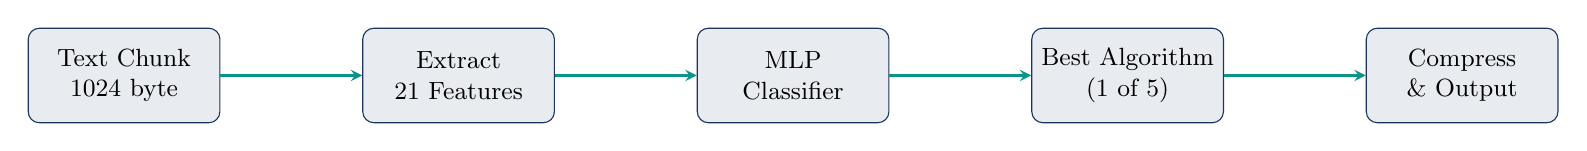
\begin{tikzpicture}[node distance=1.8cm, auto,
        block/.style={rectangle, draw=darkblue, fill=darkblue!10, text width=2.2cm, text centered, rounded corners, minimum height=1.2cm, font=\small},
        arrow/.style={->, >=stealth, thick, teal}]

      \node[block] (chunk) {Text Chunk \\ 1024 byte};
      \node[block, right=of chunk] (features) {Extract \\ 21 Features};
      \node[block, right=of features] (mlp) {MLP \\ Classifier};
      \node[block, right=of mlp] (algo) {Best Algorithm \\ (1 of 5)};
      \node[block, right=of algo] (compress) {Compress \\ \& Output};

      \draw[arrow] (chunk) -- (features);
      \draw[arrow] (features) -- (mlp);
      \draw[arrow] (mlp) -- (algo);
      \draw[arrow] (algo) -- (compress);
    \end{tikzpicture}
  \end{center}

  \vspace{0.5em}
  \begin{columns}[T]
    \column{0.5\textwidth}
    \begin{exampleblock}{Training}
      \begin{enumerate}
        \setlength{\itemsep}{0.2em}
        \item Tüm 5 algoritmayı çalıştır
        \item En iyisi = label
        \item 5-fold book-level CV
        \item MLP'yi eğit
      \end{enumerate}
    \end{exampleblock}

    \column{0.5\textwidth}
    \begin{block}{Inference}
      \begin{enumerate}
        \setlength{\itemsep}{0.2em}
        \item 21 feature çıkar (O(n))
        \item MLP inference (0.006ms)
        \item Seçilen algoritma ile sıkıştır
        \item Header: 3 bit (5 algo)
      \end{enumerate}
    \end{block}
  \end{columns}
\end{frame}

% ── Slide: Chunk Size ──
\begin{frame}{Chunk Size: Kritik Hiperparametre}
  \begin{center}
    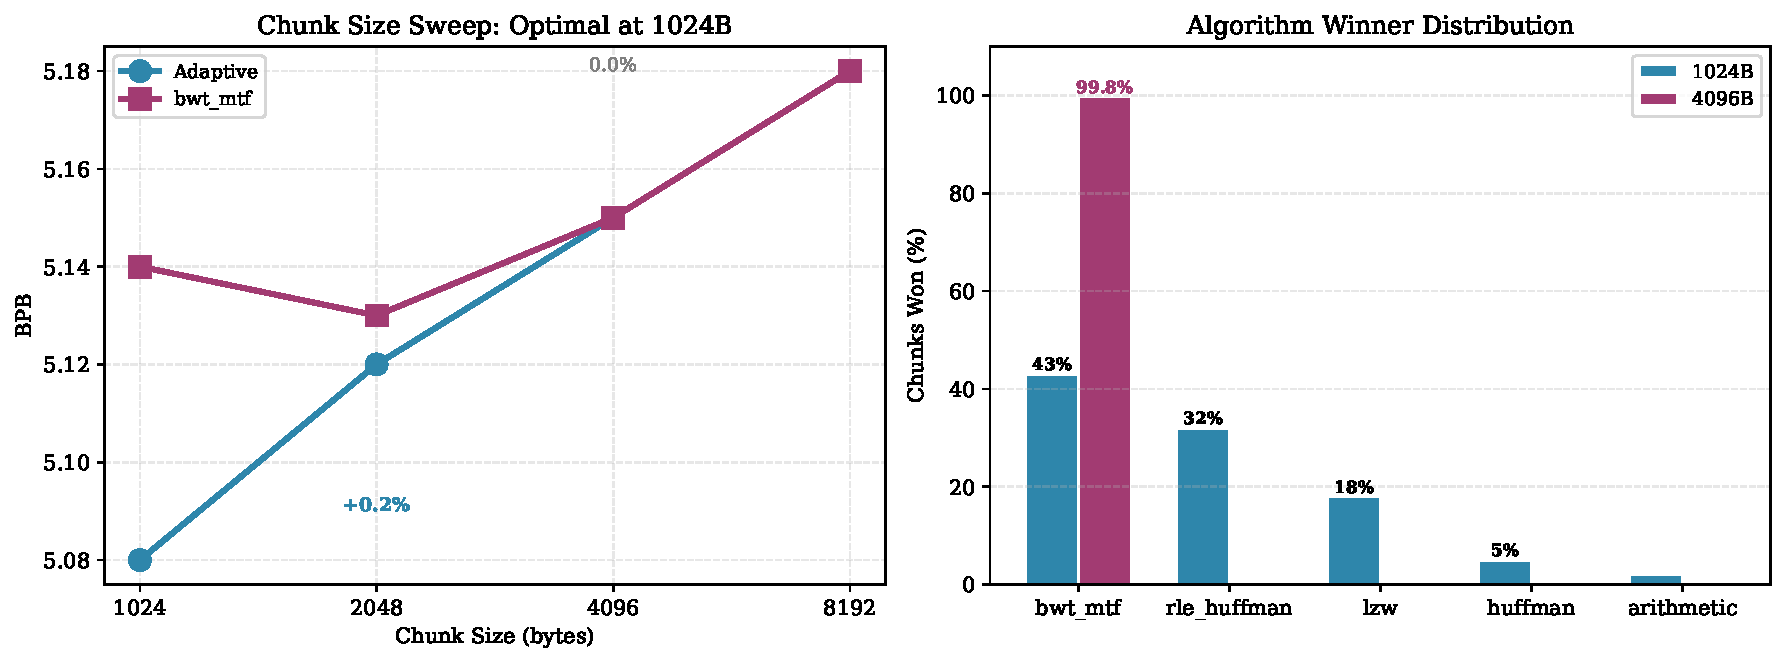
\includegraphics[width=0.82\textwidth]{figures/fig2_chunk_sweep.pdf}
  \end{center}

  \vspace{-0.3em}
  \begin{columns}[T]
    \column{0.5\textwidth}
    \begin{alertblock}{1024 byte = Sweet Spot}
      \begin{itemize}
        \setlength{\itemsep}{0.2em}
        \item 3 algoritma rekabet eder
        \item Adaptive > bwt\_mtf
      \end{itemize}
    \end{alertblock}
    \column{0.5\textwidth}
    \begin{block}{4096+ byte}
      \begin{itemize}
        \setlength{\itemsep}{0.2em}
        \item bwt\_mtf domine eder
        \item Adaptive gereksiz
      \end{itemize}
    \end{block}
  \end{columns}
\end{frame}

% ── Slide: Model Comparison ──
\begin{frame}{Model Karşılaştırması}
  \begin{center}
    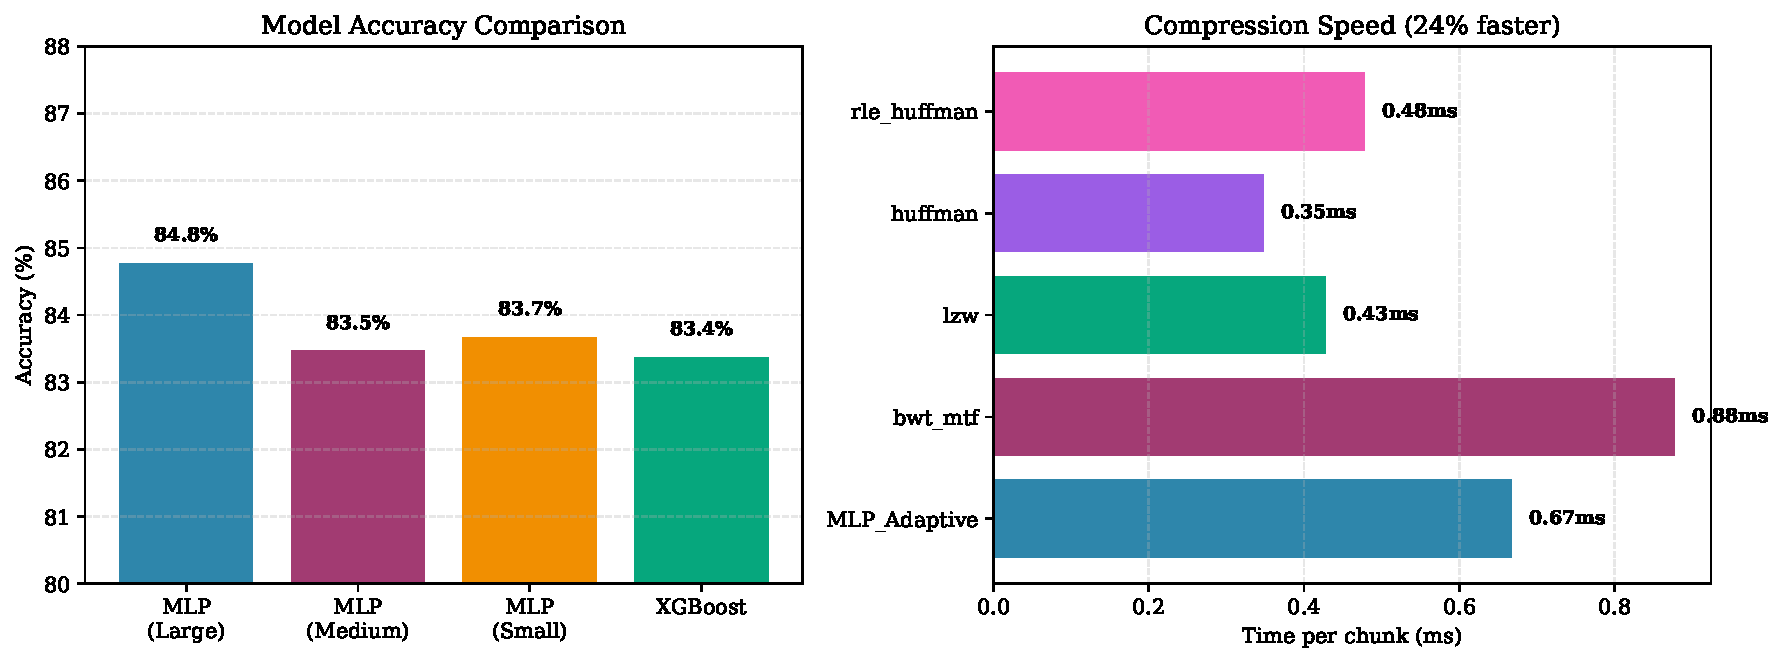
\includegraphics[width=0.82\textwidth]{figures/fig3_model_speed.pdf}
  \end{center}

  \vspace{-0.3em}
  \begin{table}
    \footnotesize
    \begin{tabular}{lccc}
      \toprule
      \textbf{Model} & \textbf{Parametre} & \textbf{Accuracy} & \textbf{Inference} \\
      \midrule
      XGBoost & 200 ağaç, d=6 & 78.2\% & 0.024ms \\
      MLP-Small & 21→32→16→3 & 79.1\% & 0.003ms \\
      MLP-Medium & 21→64→32→16→3 & 82.1\% & 0.005ms \\
      \rowcolor{teal!15} \textbf{MLP-Large} & \textbf{21→128→64→32→3} & \textbf{84.8\%} & \textbf{0.006ms} \\
      MLP-Ensemble & Soft voting (3 MLP) & 83.5\% & 0.018ms \\
      \bottomrule
    \end{tabular}
  \end{table}
\end{frame}

% ── Slide: K-Fold Results ──
\begin{frame}{K-Fold Cross-Validation Sonuçları}
  \begin{center}
    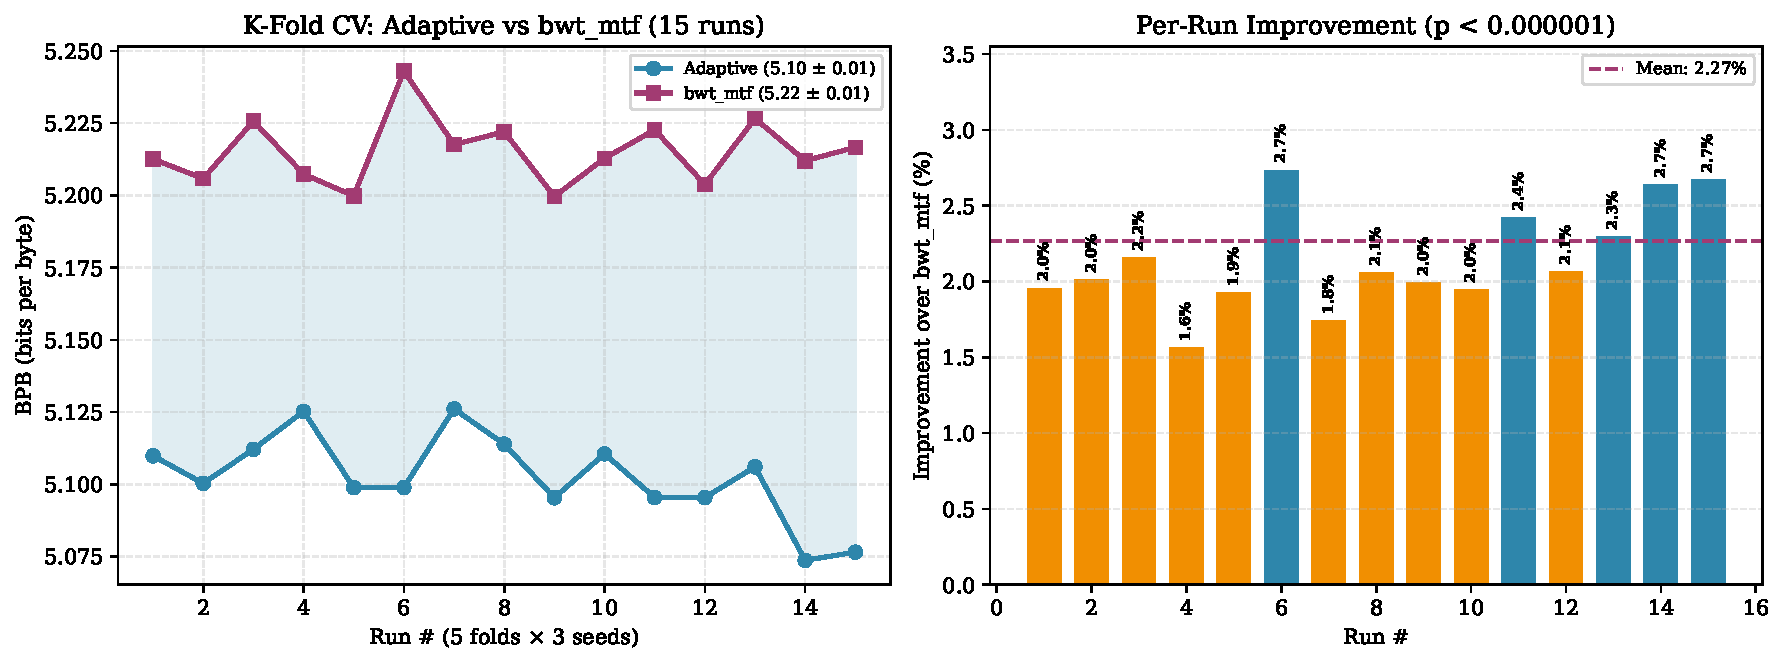
\includegraphics[width=0.82\textwidth]{figures/fig1_kfold.pdf}
  \end{center}

  \vspace{-0.5em}
  \begin{columns}[T]
    \column{0.5\textwidth}
    \begin{table}
      \footnotesize
      \begin{tabular}{lc}
        \toprule
        \textbf{Metric} & \textbf{Value} \\
        \midrule
        Adaptive BPB & \alert{5.10} \\
        bwt\_mtf BPB & 5.22 \\
        Improvement & \alert{+2.27\%} \\
        Accuracy & 82.7\% \\
        \bottomrule
      \end{tabular}
    \end{table}

    \column{0.5\textwidth}
    \begin{alertblock}{İstatistiksel Güven}
      \begin{itemize}
        \setlength{\itemsep}{0.3em}
        \item 15 run, hepsi bwt\_mtf'ten iyi
        \item $t = 43.16$
        \item \alert{$p < 10^{-6}$}
        \item Best run: +2.70\%
        \item Worst run: +1.96\%
      \end{itemize}
    \end{alertblock}
  \end{columns}
\end{frame}

% ── Slide: Oracle Gap ──
\begin{frame}{Oracle Gap: Teorik Sınıra Ne Kadar Yakınız?}
  \begin{center}
    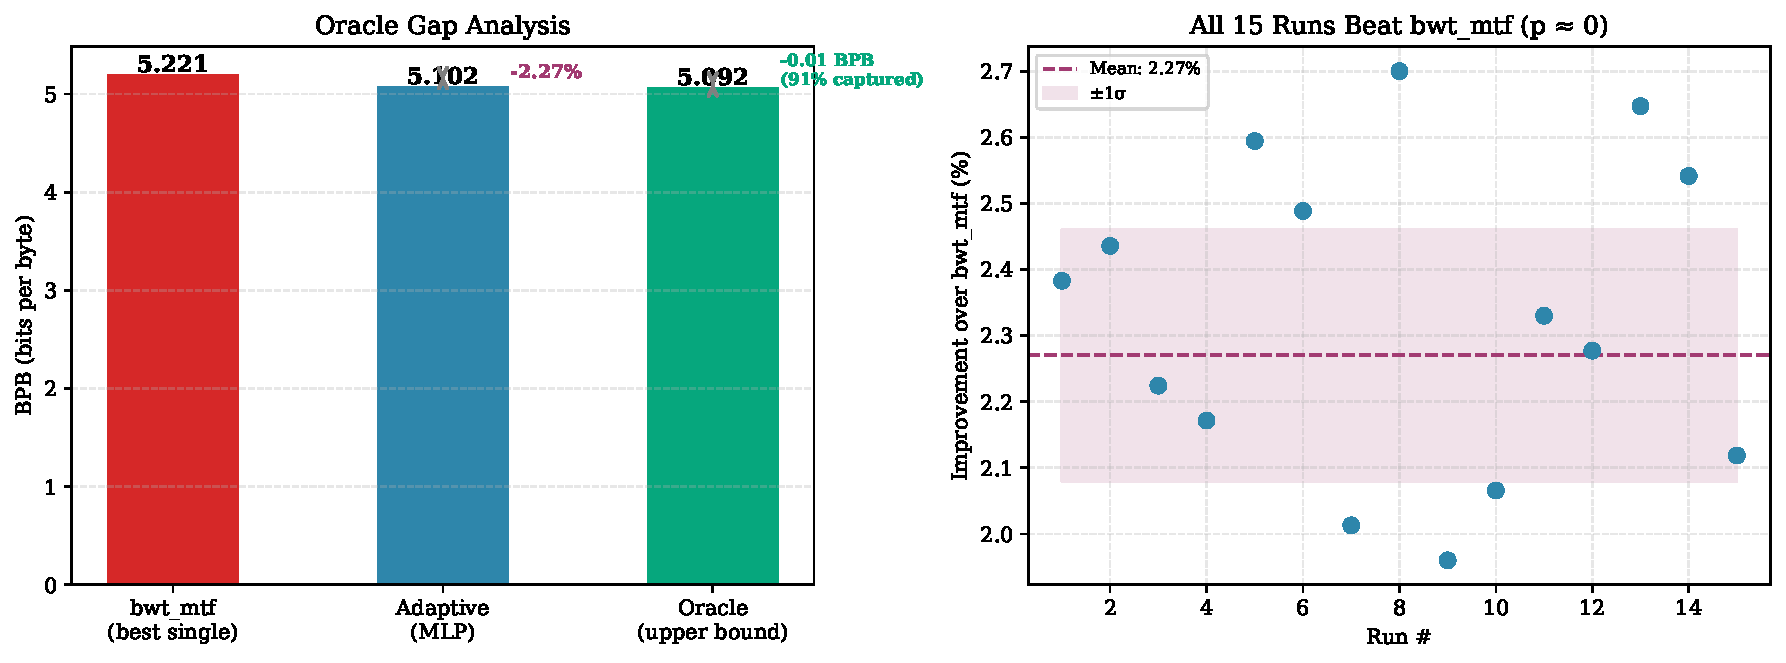
\includegraphics[width=0.82\textwidth]{figures/fig4_oracle.pdf}
  \end{center}

  \vspace{-0.5em}
  \begin{columns}[T]
    \column{0.5\textwidth}
    \begin{exampleblock}{Oracle = Mükemmel Seçici}
      \begin{itemize}
        \setlength{\itemsep}{0.3em}
        \item Oracle BPB: 5.09
        \item Adaptive BPB: 5.10
        \item Gap: \textbf{sadece 0.01 BPB}
      \end{itemize}
    \end{exampleblock}

    \column{0.5\textwidth}
    \begin{block}{Anlamı}
      \begin{itemize}
        \setlength{\itemsep}{0.3em}
        \item \textbf{\%91} teorik kazancı yakaladık
        \item \%17.3 misclassification gap
        \item Geriye kalan \textasciitilde0.01 BPB
      \end{itemize}
    \end{block}
  \end{columns}
\end{frame}

% ── Slide: Speed ──
\begin{frame}{Hız Avantajı: Daha İyi + Daha Hızlı}
  \begin{columns}[T]
    \column{0.45\textwidth}
    \begin{center}
      \textbf{Per-Chunk Zaman (ms)}
      \vspace{0.3em}

      \begin{tabular}{lr}
        \toprule
        \textbf{Algoritma} & \textbf{Süre} \\
        \midrule
        Huffman & 0.35ms \\
        LZW & 0.43ms \\
        Arithmetic & 0.51ms \\
        RLE+Huff. & 0.62ms \\
        BWT+MTF & 0.88ms \\
        \midrule
        MLP inference & 0.006ms \\
        \midrule
        \rowcolor{teal!15} \textbf{Adaptive (ort.)} & \textbf{0.67ms} \\
        \bottomrule
      \end{tabular}
    \end{center}

    \column{0.55\textwidth}
    \begin{alertblock}{Neden Daha Hızlı?}
      \begin{itemize}
        \setlength{\itemsep}{0.5em}
        \item MLP inference neredeyse bedava (0.006ms)
        \item Her zaman BWT kullanılmaz
        \item LZW/Huffman çok daha hızlı
        \item Sonuç: \textbf{\%24 daha hızlı}
      \end{itemize}
    \end{alertblock}

    \vspace{0.5em}
    \begin{block}{Header Overhead}
      5 algoritma → $\lceil\log_2(5)\rceil = 3$ bit/chunk \\
      1024 byte → $3/(1024\times8) = \textbf{\%0.037}$
    \end{block}
  \end{columns}
\end{frame}

% ── Slide: zstd ──
\begin{frame}{Modern Codec'ler: zstd Deneyi}
  \begin{alertblock}{Önemli Bulgu}
    zstd (level 3) havuza eklendiğinde \textbf{\%99.8 chunk'ta} kazanıyor.
  \end{alertblock}

  \vspace{0.5em}
  \begin{columns}[T]
    \column{0.5\textwidth}
    \textbf{Bu bir başarısızlık değil:}
    \vspace{0.3em}
    \begin{itemize}
      \setlength{\itemsep}{0.4em}
      \item Modern codec'ler klasikleri eziyor
      \item Pratikte: ``zstd kullan'' yeterli
      \item Bu \textbf{araştırma bulgusu} olarak değerli
    \end{itemize}

    \column{0.5\textwidth}
    \textbf{Projenin asıl değeri:}
    \vspace{0.3em}
    \begin{itemize}
      \setlength{\itemsep}{0.4em}
      \item Metin özellikleri $\leftrightarrow$ algoritma performansı ilişkisi
      \item Supervised ML ile routing
      \item Oracle gap: teorik limite \%91 yakınlık
    \end{itemize}
  \end{columns}
\end{frame}

% ── Slide: Discussion ──
\begin{frame}{Tartışma \& Bulgular}
  \begin{columns}[T]
    \column{0.5\textwidth}
    \begin{exampleblock}{Adaptive Ne Zaman İşe Yarar?}
      \begin{enumerate}
        \setlength{\itemsep}{0.3em}
        \item \textbf{Diverse data şart} — homojen veride tek algoritma domine eder
        \item \textbf{Doğru chunk size} — 1024B sweet spot; büyük chunk BWT'yi kayırır
      \end{enumerate}
    \end{exampleblock}

    \column{0.5\textwidth}
    \begin{alertblock}{Failure Modes}
      \begin{itemize}
        \setlength{\itemsep}{0.3em}
        \item Homojen veri: \%65 daha kötü
        \item Chunk-level leakage: \%0.26 BPB şişirme
        \item Arithmetic O1 header: 131KB → kullanılamaz
      \end{itemize}
    \end{alertblock}
  \end{columns}

  \vspace{0.5em}
  \textbf{1024 byte'ta algoritma dağılımı:}
  \vspace{0.3em}
  \begin{center}
    bwt\_mtf \%50 | rle\_huffman \%30 | lzw \%19 | \small (Huffman/Arithmetic O0 hiç kazanamaz)
  \end{center}
\end{frame}

% ═══════════════════════════════════════════════════════════════
% CONCLUSIONS
% ═══════════════════════════════════════════════════════════════
\begin{frame}{Sonuçlar}
  \begin{columns}[T]
    \column{0.55\textwidth}
    \textbf{Teknik Başarımlar:}
    \vspace{0.3em}
    \begin{enumerate}
      \setlength{\itemsep}{0.4em}
      \item MLP classifier \%82.7 accuracy
      \item \alert{\%2.27 daha iyi sıkıştırma} (vs bwt\_mtf)
      \item \alert{\%24 daha hızlı}
      \item 15/15 CV run'da kazanç ($p < 10^{-6}$)
      \item Oracle gap: 0.01 BPB (\%91 yakalama)
      \item 1024B optimal chunk size
    \end{enumerate}

    \column{0.45\textwidth}
    \textbf{AI Entegrasyonu:}
    \vspace{0.3em}
    \begin{enumerate}
      \setlength{\itemsep}{0.4em}
      \item 4 farklı AI modeli kullanıldı
      \item Agent tabanlı otonom geliştirme
      \item Supervised learning dönüşümü AI tarafından önerildi
      \item Diverse data keşfi otonom
      \item Rapor otonom yazıldı
    \end{enumerate}
  \end{columns}

  \vspace{0.5em}
  \begin{center}
    \Large\textbf{\%91 Oracle Gap + \%24 Faster + AI-Assisted + 4.83 BPB}
  \end{center}
\end{frame}

% ═══════════════════════════════════════════════════════════════
% THANK YOU
% ═══════════════════════════════════════════════════════════════
\begin{frame}[plain,c]
  \usebeamercolor[fg]{palette primary}
  \LARGE Teşekkürler \\[0.5em]
  \large Sorular? \\[1em]
  \normalsize
  \texttt{github.com/husamettinarslan/data-comp-project}
\end{frame}

\end{document}
